\documentclass[11pt, dvipsnames,aspectratio=169]{beamer}
\usetheme{Madrid}

\usepackage[utf8]{inputenc}
\usepackage{tabularray}	% for "tblr"
\usepackage{graphicx}

% Define the colors used by DNP for branding
\usepackage{xcolor}
\definecolor{dnpblue}{RGB}{0,26,174}
\definecolor{dnplightblue}{RGB}{221,226,255}
\usecolortheme[named=dnpblue]{structure}

% No navigation symbols ("next slide"/"previous slide")
\setbeamertemplate{navigation symbols}{}

% make the footline DNP blue
\setbeamercolor{palette primary}{bg=dnpblue,fg=white}
\setbeamercolor{palette secondary}{bg=dnpblue,fg=white}
\setbeamercolor{palette tertiary}{bg=dnpblue,fg=white}

% define associative array functionality, e.g.
%   \storedata\mydata{{one}{two}{three}}
%   \getdata[2]\mydata   % returns two
\newcount\tmpnum
\def\storedata#1#2{\tmpnum=0 \edef\tmp{\string#1}\storedataA#2\end}
\def\storedataA#1{\advance\tmpnum by1
	\ifx\end#1\else
	\expandafter\def\csname data:\tmp:\the\tmpnum\endcsname{#1}%
	\expandafter\storedataA\fi
}
\def\getdata[#1]#2{\csname data:\string#2:#1\endcsname}

% define the fading used on the title slide
\usepackage{tikz}
\usetikzlibrary{fadings,calc,positioning,patterns}
\tikzfading[name=dnpfading,top color=transparent!100,bottom color=transparent!100]

\tikzset{fotopunkt/.style={scale=.7,inner sep=1pt,text=white,draw=white,fill=dnpblue,circle}}
\tikzset{titlepageline/.style={anchor=north west,white,text width=4.9cm}}

% draw the zoom triangle between a point of interest and its photo
%  * number of the point (#1)
%  * photo (as a TikZ node) (#2)
\newcommand\zoomtriangle[2]{
	\tikz[remember picture,overlay]{
		\coordinate (top) at ($(map.north west)!\getdata[#1]\xcoords!(map.north east)$);
		\coordinate (bottom) at ($(map.south west)!\getdata[#1]\xcoords!(map.south east)$);
		\coordinate (target) at ($(top)!\getdata[#1]\ycoords!(bottom)$);
		\fill[gray,opacity=.35] (target) -- (#2.north west) -- (#2.south west) -- cycle;
		\node[fotopunkt] at (target) {#1};
	}
}


% bulletlist is an itemized list which has a blue bullet before each item
\setbeamertemplate{itemize items}{$\bullet$}
\newenvironment{bulletlist}[1]{\begin{itemize}\setlength{\itemsep}{#1}}{\end{itemize}}

% define a new environment "mapframe" which consists of
%  * a title (#1)
%  * a left column featuring an image (#2) of width #3
%  * a right column containing the content of the environment
% example:
% \begin{mapframe}{Frame title}{/path/to/map.png}{.5\textwidth}
	%     (content of the right column)
	% \end{mapframe}
\usepackage{environ,calc}
\NewEnviron{mapframe}[3]{\begin{frame}{#1}
		\begin{minipage}{#3}
			\tikz[remember picture]{\node[inner sep=0] (map) at (0, 0) {\includegraphics[width=\linewidth]{#2}};}
		\end{minipage}\hfill%
		\begin{minipage}{\dimexpr0.99\linewidth-#3}\BODY\end{minipage}
\end{frame}}

% logo in the bottom right corner
\logo{
\includegraphics[width=.1\textwidth]{../Bilder/Logo.png}}
\newcommand{\nologo}{\setbeamertemplate{logo}{}} % command to set the logo to nothing

\def\titlelinetwo{}
\def\titlelinethree{}

\setbeamertemplate{date}{}

\setbeamertemplate{title page}{
	\begin{tikzpicture}[overlay, remember picture, shift={(current page.south west)}]
		\node[inner sep=0pt] at (10, \paperheight/2) {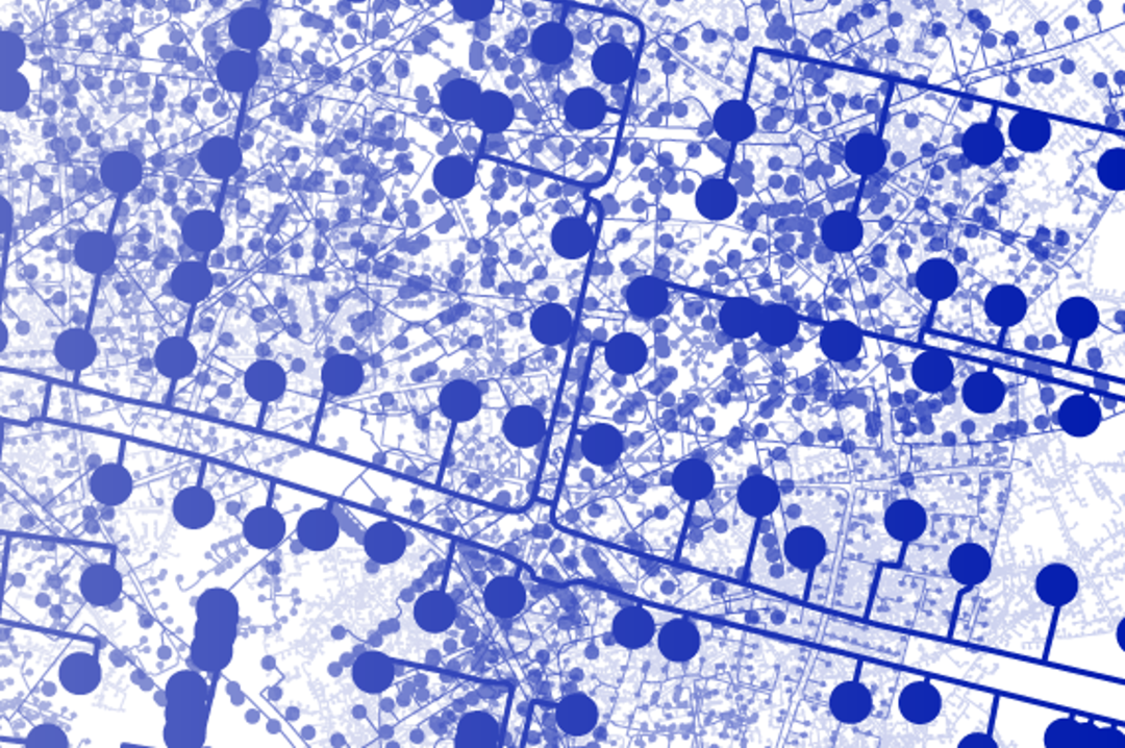
\includegraphics[height=\paperheight]{../Bilder/titelbild.pdf}};
		\fill[dnplightblue,path fading=dnpfading] (0, 0) rectangle (\paperwidth, \paperheight);
		\fill[dnpblue] (0, 0) rectangle  (5.3, \paperheight);
		\node[titlepageline] (title) at (.2, 7) {\inserttitle{}};
		\node[below=.1cm of title.south west,titlepageline,font=\scriptsize] (line2) {\titlelinetwo};
		\node[below=.1cm of line2.south west,titlepageline,font=\scriptsize] (line3) {\titlelinethree};
		\node[below=1cm of line3.south west,titlepageline,font=\scriptsize] (subtitle) {\insertsubtitle{}};
		\node[white,anchor=south west] at (.2, .2) {\tiny \insertdate{}};
		\node[anchor=south east] at (\paperwidth, .1) {\insertlogo{}};
	\end{tikzpicture}
	\addtocounter{framenumber}{-1} % exclude titlepage from page numbering
}

\makeatletter
\setbeamertemplate{footline}
{
	\leavevmode%
	\hbox{%
		\begin{beamercolorbox}[wd=.22222\paperwidth,ht=2.25ex,dp=1ex,left]{author in head/foot}%
			\usebeamerfont{author in head/foot}\hspace*{2ex}\insertshortauthor
		\end{beamercolorbox}%
		\begin{beamercolorbox}[wd=.55555\paperwidth,ht=2.25ex,dp=1ex,center]{title in head/foot}%
			\usebeamerfont{title in head/foot}\insertshorttitle
		\end{beamercolorbox}%
		\begin{beamercolorbox}[wd=.22222\paperwidth,ht=2.25ex,dp=1ex,right]{date in head/foot}%
			\usebeamerfont{date in head/foot}
			\insertframenumber{} / \inserttotalframenumber\hspace*{2ex} 
	\end{beamercolorbox}}%
	\vskip0pt%
}
\makeatother

% Ort
\newcommand{\Ort}{TODO}

% Landkreis
\newcommand{\Kreis}{TODO}

% Bundesland
\newcommand{\Land}{TODO}

% Abgabedatum
\newcommand{\Abgabedatum}{TODO}

% Kunde, z.B. GF+ oder FED
\newcommand{\Kunde}{TODO}

% Text beim Analysebeispiel für den Adresscheck
\newcommand{\adresseAnalysebeispiel}{TODO}

% Anzahl der Einheiten im Analysebeispiel
% Format: Grunddaten GF+ & Adresscheck DNP & Differenz
% Beispiel: 39 & 36 & -3
\newcommand{\einheitenAnalysebeispiel}{TODO & TODO & TODO}

% Text bei der Besonderheit beim Adresscheck
\newcommand{\besonderheitAdressen}{TODO}

% Text bei der typischen Oberfläche
\newcommand{\typischeOberflaeche}{TODO}

% Text bei der Besonderheit bei den Trenches
\newcommand{\besonderheitTrenches}{TODO}

% Text bei der Sonderquerung
\newcommand{\sonderquerung}{TODO}


\storedata\xcoords{{0}{0}{0}{0}{0}{0}}
\storedata\ycoords{{0}{0}{0}{0}{0}{0}}

\input{OberflaechenStatistik.tex}

\usepackage{eurosym}
\usepackage{adjustbox}

% square indicating classified surface
\newcommand\colorsquare[1]{\tikz{\draw[draw=black,fill=surface#1] (0, 0) rectangle (.23,.23);}}

% info shown in the footline
\author[DNP]{Deutsche Netzplanung}
\title[Ergebnisse \Ort]{\textbf{Ergebnisse} \\ \Ort}
\subtitle{Oberflächenanalyse}
\date{\Abgabedatum}


\begin{document}
	
{
	\setbeamertemplate{footline}{}
	\maketitle
}

\begin{frame}{Struktur und Inhalt der Lieferung \Ort}
	\begin{bulletlist}{5pt}
		\item Kartenüberblick inklusive von uns gezeichneter Polygone
			\begin{bulletlist}{3pt}
				\item[$\bullet$] Polygone auf Basis der von \Kunde{} gelieferten Shape-Dateien
				\item[$\bullet$] Straßen und Bürgersteige vollständig eingezeichnet und klassifiziert
				\item[$\bullet$] Eingezeichnete Flächen vollständig ausgewertet
			\end{bulletlist}
		\item Bilder aus der Kommune
		\begin{bulletlist}{3pt}
			\item[$\bullet$] Typische Bilder aus der Kernstadt
			\item[$\bullet$] Typische Bilder aus den Wohnbereichen
			\item[$\bullet$] Besondere Situation vor Ort
		\end{bulletlist}
		\item Grunddaten für Kostenanalyse
		\begin{bulletlist}{3pt}
			\item[$\bullet$] Länge der Straßenseiten: Gesamt und pro Polygon
			\item[$\bullet$] Anzahl Adressen und Haushalte
			\item[$\bullet$] Oberflächen-Aufteilung innerhalb der Polygone
			\item[$\bullet$] Anzahl und Art der Sonderquerungen
		\end{bulletlist}
	\end{bulletlist}
\end{frame}

\begin{mapframe}{Übersicht}{../Karten/karte.pdf}{.6\linewidth}
	\scriptsize
	\begin{itemize}
		\surfacetypes

		\item[\colorsquare{a}] Asphalt
		\item[\colorsquare{t}] Pflaster
		\item[\colorsquare{g}] Unbefestigt
		\item[\colorsquare{v}] Verdichtet/Schotter
		\item[\colorsquare{m}] Kopfsteinpflaster
		\item[\colorsquare{n}] kein Bürgersteig
		\item[\colorsquare{sa}] Asphaltierte Straße
		\item[\colorsquare{st}] Gepflasterte Straße
		\item[\colorsquare{sg}] Unbefestigte Straße
		\item[\colorsquare{sm}] Straße mit Kopfsteinpflaster
		\item[\colorsquare{sn}] keine öffentliche Straße
		\item[\colorsquare{sx}] Sonderquerung Straße
		\item[\colorsquare{x}] Sonderquerung
	\end{itemize}
\end{mapframe}

\begin{mapframe}{Typische Bilder}{../Karten/karte.pdf}{.55\textwidth}
	\centering
	\tikz[remember picture]{
		\node[inner sep=0] (bild1) at (0,0) {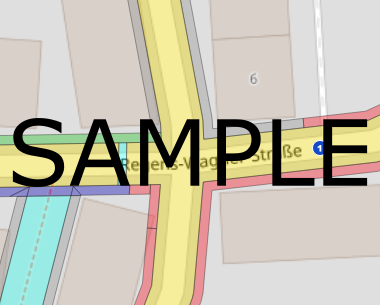
\includegraphics[width=4cm]{../Bilder/innenstadt-karte.png}};
	} \\[.3cm]
	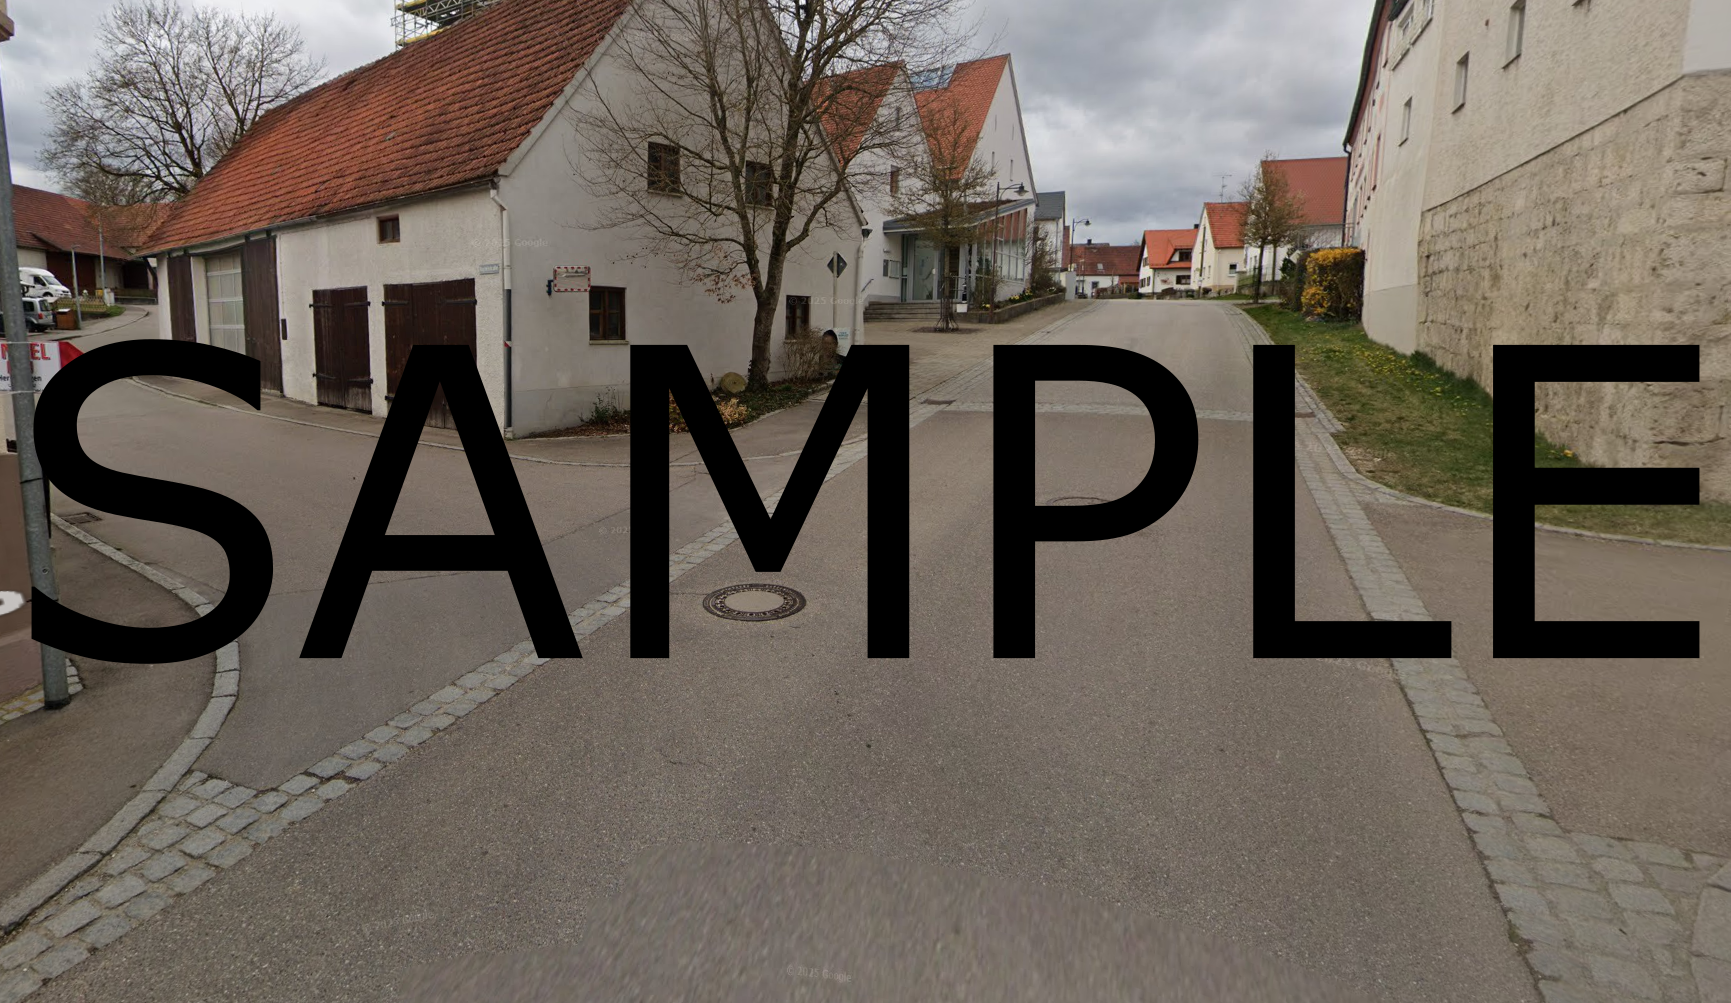
\includegraphics[width=4cm]{../Bilder/innenstadt.png} \\
	\scriptsize \bildeins
	\zoomtriangle{1}{bild1}
\end{mapframe}

\begin{mapframe}{Typische Bilder}{../Karten/karte.pdf}{.55\textwidth}
	\centering
	\tikz[remember picture]{
		\node[inner sep=0] (bild2) at (0,0) {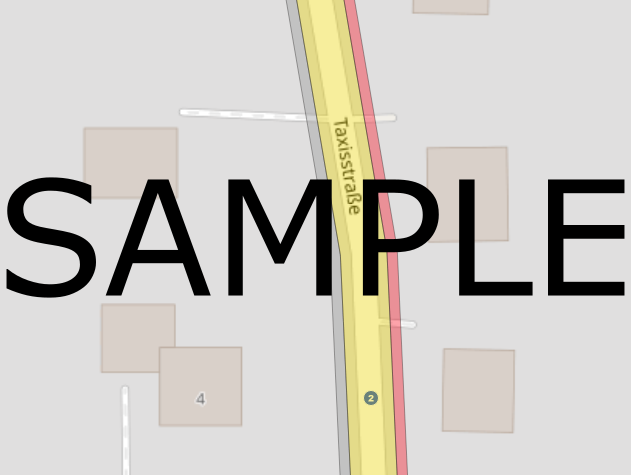
\includegraphics[width=4cm]{../Bilder/wohnsiedlung-karte.png}};
	} \\[.3cm]
	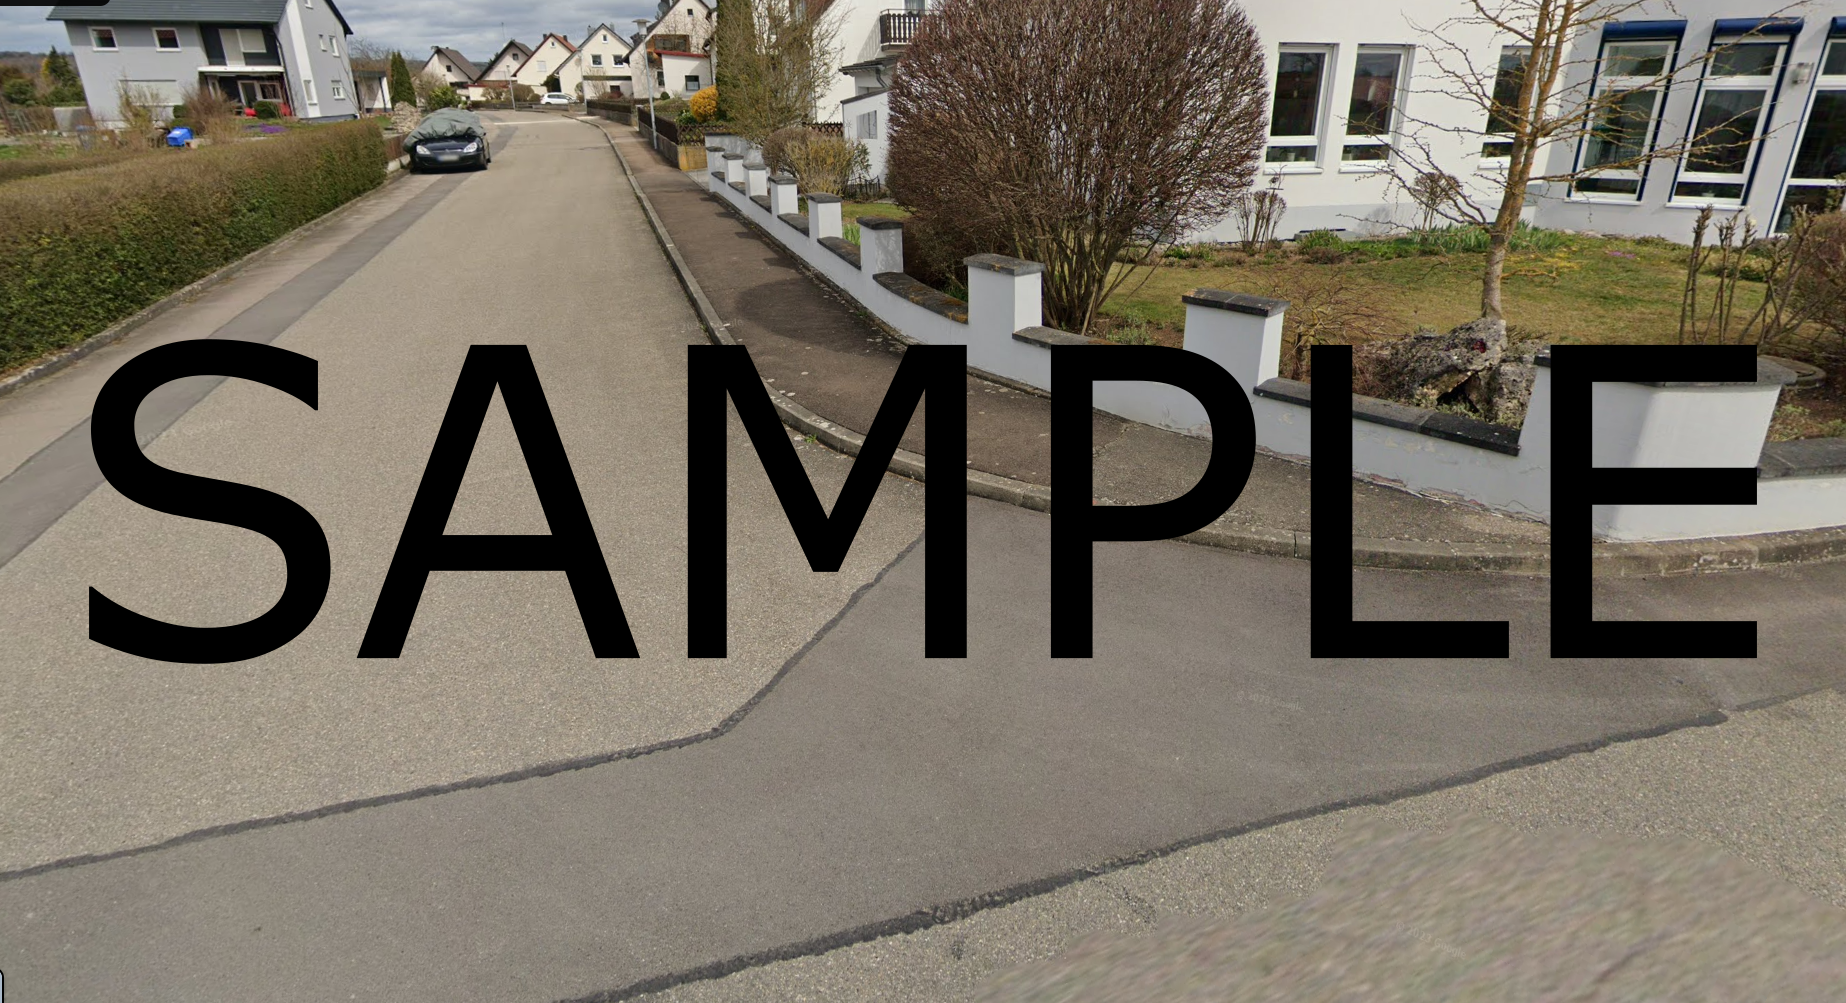
\includegraphics[width=4cm]{../Bilder/wohnsiedlung.png} \\
	\scriptsize \bildzwei
	\zoomtriangle{2}{bild2}
\end{mapframe}

\begin{mapframe}{Besonderheit}{../Karten/karte.pdf}{.55\textwidth}
	\centering
	\tikz[remember picture]{
		\node[inner sep=0] (bild3) at (0,0) {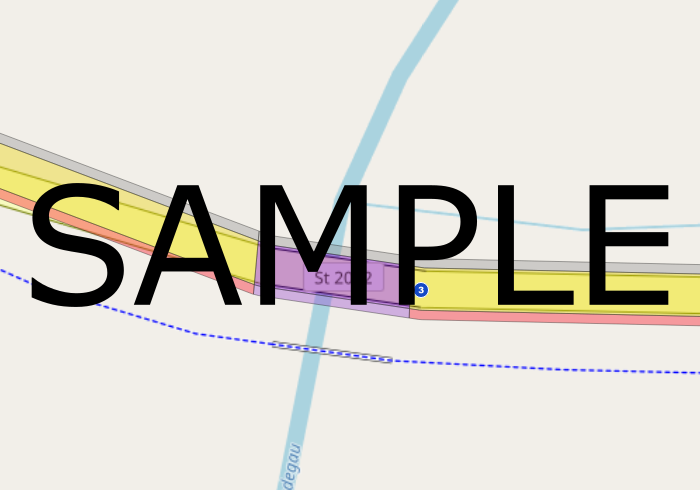
\includegraphics[width=4cm]{../Bilder/besonderheit-karte.png}};
	} \\[.3cm]
	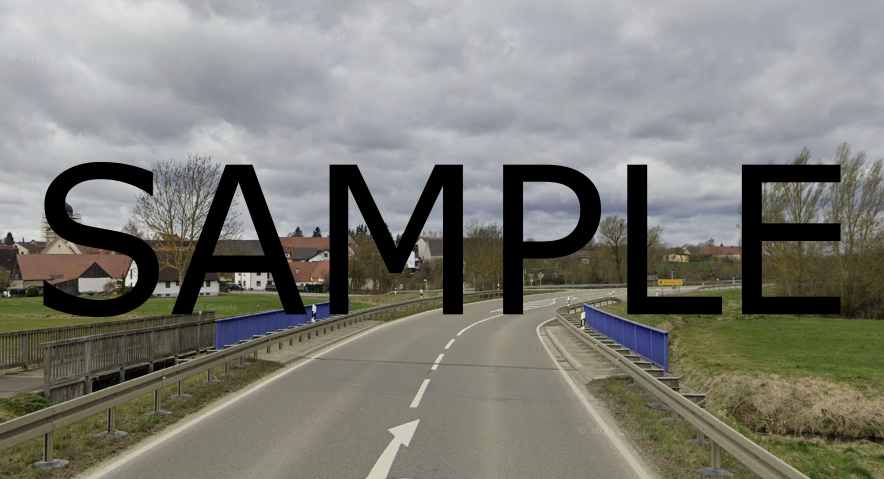
\includegraphics[width=4cm]{../Bilder/besonderheit.png} \\
	\scriptsize \bilddrei
	\zoomtriangle{3}{bild3}
\end{mapframe}

\begin{frame}[t]{Grunddaten für Kostenanalyse}
	\scriptsize

	\adjustbox{valign=t}{\begin{minipage}{.47\textwidth}
		\begin{tblr}{width=\textwidth,colspec={l@{}Xrr},row{1}={bg=dnpblue,fg=white,font=\bfseries},row{8}={font=\bfseries}}
			& Oberfläche Bürgersteige & Länge & Anteil \\
			\colorsquare{g}\hspace{5pt} & Unbefestigt & 19845~m & 43~\% \\
			\colorsquare{v} & Verdichtet & 19845~m & 43~\% \\
			\colorsquare{t} & Pflaster & 19845~m & 43~\% \\
			\colorsquare{a} & Asphalt & 19845~m & 43~\% \\
			\colorsquare{m} & Kopfstein-/Mosaikpflaster & 19845~m & 43~\% \\
			\colorsquare{n} & kein Bürgersteig & 19845~m & 43~\% \\
			& Gesamt & 19845~m & 100~\% \\
		\end{tblr}
		\end{minipage}}\hfill%
	\adjustbox{valign=t}{\begin{minipage}[t]{.52\textwidth}
		\begin{tblr}{width=\textwidth,colspec={l@{}X[l]rrr},row{1}={bg=dnpblue,fg=white,font=\bfseries},row{4}={font=\bfseries}}
			& Sonderquerungen & Länge & Anteil & Anzahl \\
			& Bach-, Flussquerung Bürgersteig & 62~m & 63~\% & 2 \\
			& Bach-, Flussquerung Straße & 37~m & 37~\% & 1 \\
			& Gesamt & 99~m & 100~\% & 3 \\
		\end{tblr}
	\end{minipage}}
	
	\adjustbox{valign=t}{\begin{minipage}[t]{.47\textwidth}
		\begin{tblr}{width=\textwidth,colspec={l@{}Xrr},row{1}={bg=dnpblue,fg=white,font=\bfseries},row{7}={font=\bfseries}}
			& Oberfläche Straße & Länge & Anteil \\
			\colorsquare{sg}\hspace{5pt} & Unbefestigte Straße & 23~m & 43~\% \\
			\colorsquare{st} & Gepflasterte Straße & 12~m & 43~\% \\
			\colorsquare{sa} & Asphaltierte Straße & 124~m & 43~\% \\
			\colorsquare{sm} & Straße mit Kopfsteinpflaster & 234~m & 43~\% \\
			& nicht BIS-geeignet & 2000~m & 43~\% \\
			& Gesamt & 5000~m & 100~\% \\
		\end{tblr}
	\end{minipage}}\hfill%
	\adjustbox{valign=t}{\begin{minipage}[t]{.52\textwidth}
		\begin{tblr}{width=\textwidth,colspec={l@{}Xrr},row{1}={bg=dnpblue,fg=white,font=\bfseries},row{4}={font=\bfseries}}
			& Gesamtoberfläche & Länge & Anteil \\
			& Bürgersteig & 19845~m & 43~\% \\
			& Straße 	  & 19845~m & 43~\% \\
			& Gesamt	  & 19845~m & 100~\% \\
		\end{tblr}
	\end{minipage}}
\end{frame}

\begin{frame}{Preise \Ort}
	\begin{itemize}
		\setlength{\itemsep}{5pt} 
		\item Kommerzielles Modell
		\begin{itemize}
			\item[$\bullet$] Analysierte Straßenmeter mit einem Preis von $0.21~\text{\euro}$ pro Meter
			\item[$\bullet$] Kosten für \Ort: 1000 m $\:\times$ $0.21~\frac{\text{\euro}}{m} = 210~\text{\euro}$
			%\item[$\bullet$] Nicht rechnungsrelevant: $\Differenz$ m $\:\times$ $0\euro$ = $0\euro$
			\begin{itemize}
				\item[$\bullet$] \Ort{} - Ziertheim: $24.401$m
				%\item[$\bullet$] \Ort - Polygon: $yyy$m	
				%\item[$\bullet$] \Ort - Polygon: $yyy$m
				%\item[$\bullet$] \Ort - Polygon: $yyy$m
				%\item[$\bullet$] \Ort - Polygon: $yyy$m
				%\item[$\bullet$] \Ort - Polygon: $yyy$m
				%\item[$\bullet$] \Ort - Polygon: $yyy$m
				%\item[$\bullet$] \Ort - Polygon: $yyy$m			
				%\item[$\bullet$] \Ort - Polygon: $yyy$m
				%\item[$\bullet$] \Ort - Polygon: $yyy$m
			\end{itemize}
		\end{itemize}
		\item Timing
		\begin{itemize}
			\item[$\bullet$] Abgabe am \Abgabedatum
		\end{itemize}
	\end{itemize}
\end{frame}


\end{document}